% Digital Logic Report Template
% Created: 2020-01-10, John Miller

%==========================================================
%=========== Document Setup  ==============================

% Formatting defined by class file
\documentclass[11pt]{article}

% ---- Document formatting ----
\usepackage[margin=1in]{geometry}	% Narrower margins
\usepackage{booktabs}				% Nice formatting of tables
\usepackage{graphicx}				% Ability to include graphics

%\setlength\parindent{0pt}	% Do not indent first line of paragraphs 
\usepackage[parfill]{parskip}		% Line space b/w paragraphs
%	parfill option prevents last line of pgrph from being fully justified

% Parskip package adds too much space around titles, fix with this
\RequirePackage{titlesec}
\titlespacing\section{0pt}{8pt plus 4pt minus 2pt}{3pt plus 2pt minus 2pt}
\titlespacing\subsection{0pt}{4pt plus 4pt minus 2pt}{-2pt plus 2pt minus 2pt}
\titlespacing\subsubsection{0pt}{2pt plus 4pt minus 2pt}{-6pt plus 2pt minus 2pt}

% ---- Hyperlinks ----
\usepackage[colorlinks=true,urlcolor=blue]{hyperref}	% For URL's. Automatically links internal references.

% ---- Code listings ----
\usepackage{listings} 					% Nice code layout and inclusion
\usepackage[usenames,dvipsnames]{xcolor}	% Colors (needs to be defined before using colors)

% Define custom colors for listings
\definecolor{listinggray}{gray}{0.98}		% Listings background color
\definecolor{rulegray}{gray}{0.7}			% Listings rule/frame color

% Style for Verilog
\lstdefinestyle{Verilog}{
	language=Verilog,					% Verilog
	backgroundcolor=\color{listinggray},	% light gray background
	rulecolor=\color{blue}, 			% blue frame lines
	frame=tb,							% lines above & below
	linewidth=\columnwidth, 			% set line width
	basicstyle=\small\ttfamily,	% basic font style that is used for the code	
	breaklines=true, 					% allow breaking across columns/pages
	tabsize=3,							% set tab size
	commentstyle=\color{gray},	% comments in italic 
	stringstyle=\upshape,				% strings are printed in normal font
	showspaces=false,					% don't underscore spaces
}

% How to use: \Verilog[listing_options]{file}
\newcommand{\Verilog}[2][]{%
	\lstinputlisting[style=Verilog,#1]{#2}
}




%======================================================
%=========== Body  ====================================
\begin{document}


\title{ELC 2137 Lab 9: ALU}
\author{Jake Simmons}

\maketitle


\section*{Summary}

The purpose of this lab was to create an Arithmetic Logic Unit capable of operations. As well as explore the ideas of combinational and regular sequentional logic in SR Latches, D Latches, D flip-flop and D registers. In this lab, a Register module was created and succesfully tested. An ALU module was created and succesfully tested.  


\section*{Q\&A}



\section*{Results}

\begin{figure}[ht]\centering
	\begin{tabular}{l|rrrrrrrrrrr}
		Time (ns): & 0-5 & 5-10 & 10-15 & 15-20 & 20-25 & 25-30 & 30-35 & 35-40 & 40-45 & 45-50 & 50-55 \\
		\midrule
		D (hex) & 0 & 0 & A & A & 3 & 3 & 0 & 0 & 0$\rightarrow$6 & 6 & 6 \\
		clk & 0 & 1 & 0 & 1 & 0 & 1 & 0 & 1 & 0 & 1 & 0  \\
		en & 0 & 0 & 1 & 1 & 1$\rightarrow$0 & 0$\rightarrow$1 & 1$\rightarrow$0 & 0 & 0$\rightarrow$1 & 1 & 1 \\
		rst & 0 & 0$\rightarrow$1 & 0 & 0 & 0 & 0 & 0 & 0 & 0 & 0 & 0 \\
		\midrule 
		Q (hex) & X & X$\rightarrow$0 & 0 & A & A & A & A & A & A & 6 & 6 \\
		\bottomrule
	\end{tabular}\medskip
	
	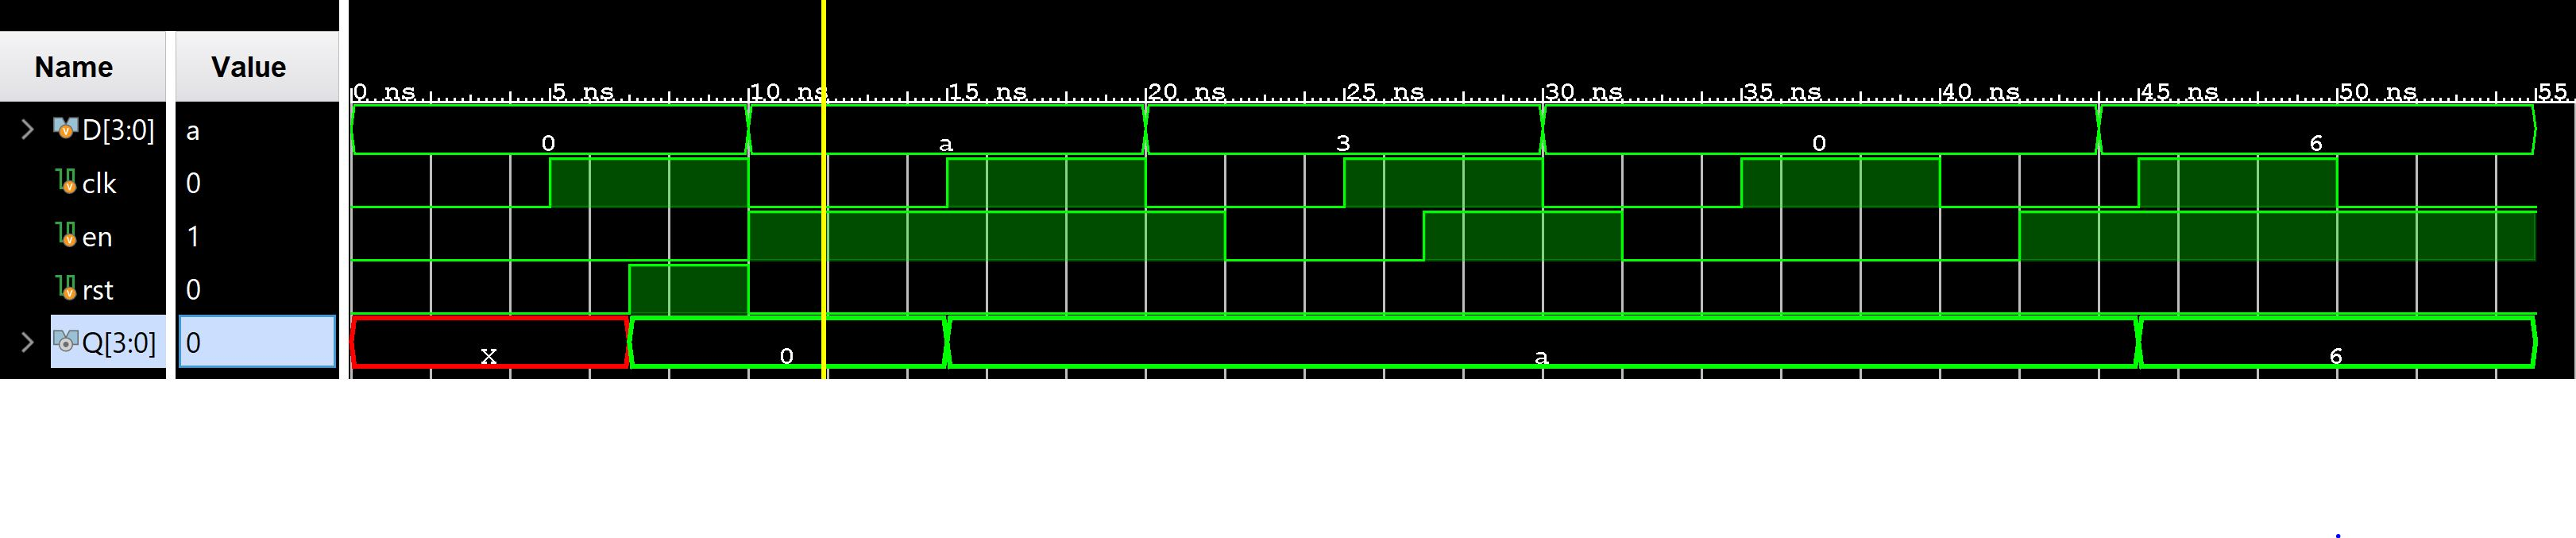
\includegraphics[width=0.95\textwidth]{register_test.JPG}
	\caption{ERT and Simultion Waveforms of Register}
	\label{fig:sim_with_table}
\end{figure}

\begin{figure}[ht]\centering
	\begin{tabular}{l|rrrrrr}
		Time (ns): & 0-10 & 10-20 & 20-30 & 30-40 & 40-50 & 50-60  \\
		\midrule
		in0 (dec) & 5 & A & 1 & 3 & 5 & F \\
		in1 (dec) & 5 & 5 & 2 & 4 & 6 & C \\
		op (dec) & 0 & 1 & 2 & 3 & 4 & 5 \\
		\midrule 
		out (dec) & A & 5 & 0 & 7 & 3 & F \\
		\bottomrule
	\end{tabular}\medskip
	
		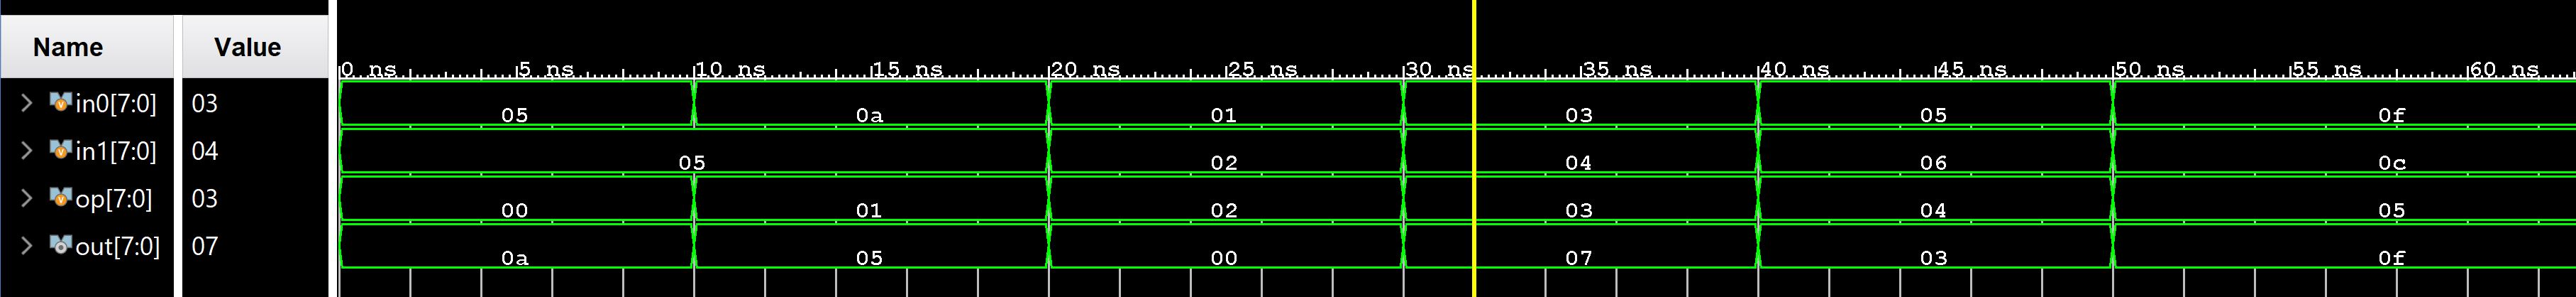
\includegraphics[width=0.95\textwidth]{ALU_test.JPG}
		\caption{ERT and Simulation Waveforms of ALU}
		\label{fig:sim_with_table}
\end{figure}

\begin{figure}[ht]\centering
	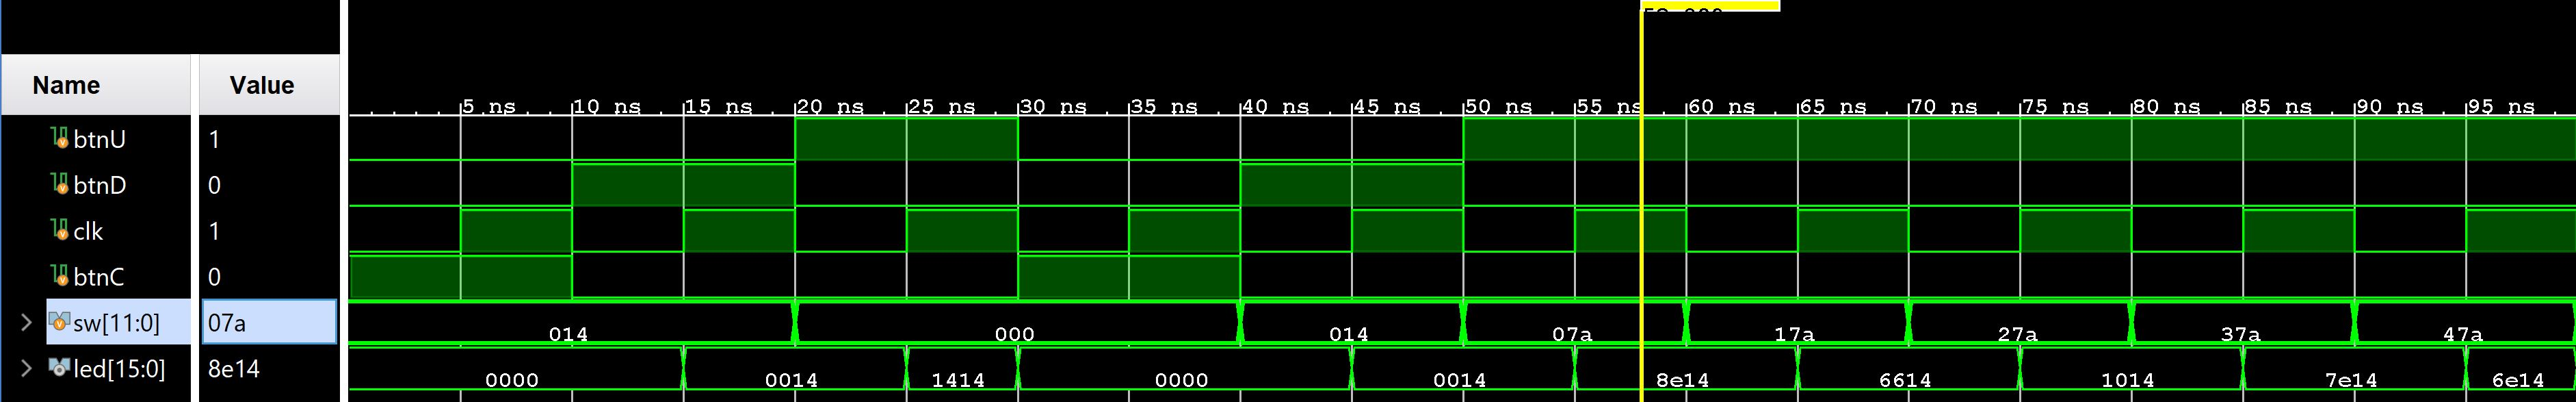
\includegraphics[width=0.95\textwidth]{top_module_test.JPG}
	\caption{Top Level Simulation Waveforms}
	\label{fig:sim}
	
\end{figure}


\clearpage
\section*{Code}

\begin{lstlisting}[style=Verilog,
caption=Register Module,
label=register 
]
`timescale 1ns / 1ps
//ELC 2137 Jake Simmons 2020-3-26

module register_2 #(parameter N=1) 
	(
	input clk, rst, en, 
	input [N-1:0] D, 
	output reg [N-1:0] Q 
	);
	always @(posedge clk, posedge rst) 
		begin       
			if (rst==1) 
				Q <= 0'b0 ; 
			else if (en==1) 
				Q <= D ; 
	end
	// Notes: // - Reset is asynchronous , so this 
	// block needs to execute when rst 
	// goes high.
	// - We want enable to be synchronous 
	// (i.e. only happens on rising 
	// edge of clk), so it is left out 
	// of "sensitivity" list.
endmodule

\end{lstlisting}

\begin{lstlisting}[style=Verilog,
caption=ALU Module,
label=ALU 
]
`timescale 1ns / 1ps
//ELC 2137 Jake Simmons 2020-3-29

module ALU#(parameter N=8) 
	( 
	output reg[N-1:0] out, 
	input [N-1:0] in0, 
	input [N-1:0] in1, 
	input [3:0] op 
	);
	// Local parameters 
	parameter ADD=0; 
	parameter SUB=1; 
	parameter AND=2; 
	parameter OR=3; 
	parameter XOR=4;

	always @* 
		begin 
			case(op) 
				ADD: out = in0 + in1; 
				SUB: out = in0 - in1;
				AND: out = in0 & in1;
				OR:  out = in0 | in1;
				XOR: out = in0 ^ in1;
				default: out = in0; 
			endcase 
		end
endmodule

\end{lstlisting}

\begin{lstlisting}[style=Verilog,
caption=Lab 9 Top Module,
label=Top
]
`timescale 1ns / 1ps
//ELC 2137 Jake Simmons 2020-3-30


module top_lab9(
	input btnU,
	input btnD,
	input [11:0] sw,
	input clk,
	input btnC,
	output [15:0] led
	);
	wire [7:0] W1;
	wire [7:0] W2;

	register_2 #(.N(8)) r1( .D(sw[7:0]), .en(btnD), .clk(clk), .Q(W1), .rst(btnC)
	);

	ALU alu( .in1(W1), .in0(sw[7:0]), .op(sw[11:8]), .out(W2)
	);

	register_2 #(.N(8)) r2( .D(W2), .en(btnU), .clk(clk), .rst(btnC), .Q(led[15:8])
	);

	assign led [7:0] = W1;
endmodule

\end{lstlisting}

\begin{lstlisting}[style=Verilog,
caption=Register Test Bench Code,
label=Register_Test
]
`timescale 1ns / 1ps
//ELC 2137 Jake Simmons 2020-3-26

module register_2_test();

	reg [3:0] D;
	reg clk, en, rst; 
	wire [3:0] Q;
	register_2 #(.N(4)) r(.D(D), .clk(clk), 
	.en(en), .rst(rst), .Q(Q) );

	// clock runs continuously 
	always begin 
		clk = ~clk; #5; 
	end
	// this block only runs once 
	initial begin
		clk = 0; en = 0; rst = 0; D = 4'h0; #7;
		rst = 1; #3; // reset 
		D = 4'hA; en = 1; rst = 0; #10; 
		D = 4'h3; #2; 
		en = 0; #5; 
		en = 1; #3;
		D = 4'h0; #2; 
		en = 0; #10; 
		en = 1; #2; 
		D = 4'h6; #11;
		$finish;
	end
endmodule

\end{lstlisting}

\begin{lstlisting}[style=Verilog,
caption=ALU Test Bench Code,
label=ALU_Test 
]
`timescale 1ns / 1ps
//ELC 2137 Jake Simmons 2020-3-29

module ALU_Test();
	reg [7:0] in0;
	reg [7:0] in1;
	reg [7:0] op;
	wire [7:0] out;

	ALU alu(
	.in0(in0), .in1(in1), .op(op), .out(out)
	);
	initial 
		begin
			in0 = 8'd5; in1 = 8'd5; op = 0; #10;
			in0 = 8'd10; in1 = 8'd5; op = 1; #10;
			in0 = 8'd1; in1 = 8'd2; op = 2; #10;
			in0 = 8'd3; in1 = 8'd4; op = 3; #10;
			in0 = 8'd5; in1 = 8'd6; op = 4; #10;
			in0 = 8'd15; in1 = 8'd12; op = 5; #10;
		end
endmodule
\end{lstlisting}


\end{document}
